\documentclass[11pt]{article}
\usepackage[margin=2.5cm]{geometry}
\usepackage{amsmath,amssymb,amsthm}
\usepackage{graphicx}
\usepackage{booktabs}
\usepackage{hyperref}
\usepackage{xcolor}
\usepackage{listings}
\usepackage{microtype}
\usepackage{caption}
\usepackage{float}

\lstset{
  basicstyle=\ttfamily\small,
  showstringspaces=false,
  breaklines=true,
  frame=single,
  framesep=3pt,
  xleftmargin=6pt,
  xrightmargin=6pt,
}

\newtheorem{proposition}{Proposition}
\theoremstyle{definition}
\newtheorem{definition}{Definition}

\title{\textbf{Milestone M1: \texttt{FourierSeries.jl}}\\[0.4em]
\large Exact Interval-Arithmetic Trig Polynomial Library\\[0.2em]
\normalsize \texttt{wave-cap} --- Computer-Assisted Proof for the Babenko Equation}
\author{BabenkoRigorous.jl}
\date{May 2026}

\begin{document}
\maketitle

\begin{abstract}
We describe the implementation and validation of \texttt{FourierSeries.jl}, the
foundational arithmetic layer of the \texttt{BabenkoRigorous.jl} Julia package.
The module provides exact interval-arithmetic operations on finite trigonometric
polynomials using the \texttt{Arblib.jl} library (FLINT/Arb ball arithmetic).
All five milestone tests pass: the Hilbert transform squares to $-I$, commutes
with differentiation, satisfies the product rule, and the supremum-norm bound
is verified to contain the true function value at 1000 grid points. Arb and
Float64 computations agree to better than $10^{-13}$.
\end{abstract}

\tableofcontents
\bigskip

%% ─────────────────────────────────────────────────────────────────────────────
\section{Background and motivation}

The long-term goal of \texttt{wave-cap} is a \emph{computer-assisted proof} (CAP)
that rigorously bounds the residual of the Babenko equation with surface tension:
\begin{equation}\label{eq:babenko}
  \mu \hat H[y_u]
  = y + y\hat H[y_u] + \hat H(y y_u)
    - \beta\,\partial_u\!\left(\frac{y_u}{D}\right)
    + \beta\,\hat H\!\left[\partial_u\!\left(\frac{1+\hat H[y_u]}{D}\right)\right],
\end{equation}
where $D = \sqrt{y_u^2 + (1+\hat H[y_u])^2}$ and $\hat H$ is the
\emph{periodic Hilbert transform}.
Given an approximate solution $y(u) = \sum_{k=1}^N a_k \cos(ku)$, we want a
certified bound $\|R\|_{L^\infty([0,2\pi])} \le \varepsilon$ on the residual
$R = \mathrm{LHS} - \mathrm{RHS}$.

The CAP has two components:
\begin{itemize}
  \item \textbf{Julia} (\texttt{BabenkoRigorous.jl}): computes the certificate
        $(\varepsilon_0, L, D_{\min}, M_{\mathrm{grid}})$ using Arb ball arithmetic.
  \item \textbf{Lean 4} (\texttt{BabenkoWave}): proves that the certificate implies
        $\|R\|_\infty \le \varepsilon_0 + L\pi/M_{\mathrm{grid}}$.
\end{itemize}

Milestone M1 delivers the foundational Julia building block: exact arithmetic on
finite trigonometric polynomials with Arb coefficients.

%% ─────────────────────────────────────────────────────────────────────────────
\section{Mathematical content}

\subsection{Trigonometric polynomials}

\begin{definition}
A \emph{trigonometric polynomial of degree $N$} is a function
\[
  f(u) = \frac{a_0}{2} + \sum_{k=1}^N \bigl(a_k \cos(ku) + b_k \sin(ku)\bigr),
  \qquad u \in [0, 2\pi].
\]
We store it as two coefficient vectors $(a_0,\ldots,a_N)$ and $(b_0,\ldots,b_N)$
with $b_0 = 0$ always.
\end{definition}

\subsection{The periodic Hilbert transform}

The periodic Hilbert transform $\hat H : L^2([0,2\pi]) \to L^2([0,2\pi])$
is defined on Fourier modes by
\[
  \hat H[e^{iku}] = -i\,\operatorname{sgn}(k)\,e^{iku},
\]
which on cosine/sine basis functions gives
\begin{align}
  \hat H[\cos(ku)] &= \sin(ku), \label{eq:Hcos}\\
  \hat H[\sin(ku)] &= -\cos(ku), \label{eq:Hsin}\\
  \hat H[1] &= 0. \label{eq:HDC}
\end{align}
For $f$ a finite trigonometric polynomial, $\hat H[f]$ is computed
\emph{exactly} by applying \eqref{eq:Hcos}--\eqref{eq:HDC} mode by mode.

\subsection{Key algebraic identities}

The following hold for smooth $2\pi$-periodic functions and are verified
computationally in M1:
\begin{align}
  \hat H^2[f] &= -f \quad (\text{on mean-zero functions}), \label{eq:Hsq}\\
  \partial_u \hat H[f] &= \hat H[\partial_u f]. \label{eq:commute}
\end{align}

\subsection{Supremum-norm bound}

For a trigonometric polynomial $f(u) = \frac{a_0}{2} + \sum_k (a_k\cos ku + b_k\sin ku)$,
\begin{equation}\label{eq:bernstein}
  \|f\|_{L^\infty} \le \frac{|a_0|}{2} + \sum_{k=1}^N \bigl(|a_k| + |b_k|\bigr).
\end{equation}
This follows from the triangle inequality and $|\cos(ku)| \le 1$, $|\sin(ku)| \le 1$.
It is the $\ell^1$-norm of the Fourier coefficients, and is an $O(1)$-tight bound
(tight when all modes are in phase).

%% ─────────────────────────────────────────────────────────────────────────────
\section{Implementation}

\subsection{The \texttt{TrigPoly} struct}

\begin{lstlisting}
struct TrigPoly
    a :: Vector{Arb}   # a[k+1] = coefficient of cos(ku), k = 0..N
    b :: Vector{Arb}   # b[k+1] = coefficient of sin(ku), k = 0..N; b[1] = 0
    prec :: Int        # Arb working precision in bits
end
\end{lstlisting}

Every coefficient is an \texttt{Arb} ball $[m \pm r]$ (midpoint plus radius),
so all arithmetic carries certified error enclosures.

\subsection{Core operations}

\paragraph{Hilbert transform (\texttt{hilbert}).}
Applies \eqref{eq:Hcos}--\eqref{eq:HDC} in $O(N)$ time:
\begin{lstlisting}
function hilbert(f::TrigPoly)::TrigPoly
    g = TrigPoly(copy(f.a), copy(f.b), f.prec)
    g.a[1] = Arb(0; prec=f.prec)          # H[const] = 0
    for k in 1:degree(f)
        g.b[k+1] =  f.a[k+1]              # cos(ku) -> sin(ku)
        g.a[k+1] = -f.b[k+1]              # sin(ku) -> -cos(ku)
    end
    return g
end
\end{lstlisting}

\paragraph{Derivative (\texttt{deriv}).}
Applies $\partial_u\cos(ku) = -k\sin(ku)$ in $O(N)$ time.

\paragraph{Product (\texttt{*}).}
Uses the four product-to-sum identities:
\begin{align*}
  \cos(ju)\cos(ku) &= \tfrac{1}{2}[\cos((j{-}k)u) + \cos((j{+}k)u)],\\
  \sin(ju)\sin(ku) &= \tfrac{1}{2}[\cos((j{-}k)u) - \cos((j{+}k)u)],\\
  \cos(ju)\sin(ku) &= \tfrac{1}{2}[\sin((j{+}k)u) - \sin((j{-}k)u)],\\
  \sin(ju)\cos(ku) &= \tfrac{1}{2}[\sin((j{+}k)u) + \sin((j{-}k)u)].
\end{align*}
The output has degree $\deg f + \deg g$ and requires $O(N^2)$ Arb
multiplications. The DC term ($k=0$, i.e.\ $\cos(0\cdot u)=1$) is handled
separately.

\paragraph{Evaluation (\texttt{tp\_eval}).}
Evaluates $f$ at an \texttt{Arb} point $u$ by summing all terms using
Arblib's certified $\cos$ and $\sin$.

\paragraph{Supremum bound (\texttt{supnorm\_bound}).}
Returns the right-hand side of \eqref{eq:bernstein} as an \texttt{Arb} ball.

\subsection{Convenience constructors}

\begin{lstlisting}
# Build a pure cosine series from Float64 coefficients
# coeffs[k] is the coefficient of cos(ku)
cosine_series(coeffs::Vector{Float64}; prec=128) -> TrigPoly
\end{lstlisting}
Each \texttt{Float64} is converted exactly to \texttt{Arb} (every
\texttt{Float64} is a dyadic rational and is representable exactly in Arb).

%% ─────────────────────────────────────────────────────────────────────────────
\section{Tests and results}

\subsection{Test T1.1: $\hat H^2 = -I$}

For a random degree-8 trigonometric polynomial $f$ (seeded for reproducibility),
we verify that all coefficients of $\hat H(\hat H(f)) + f$ have Arb balls
containing zero.

\begin{lstlisting}
f = random_trigpoly(8; seed=42)
g = hilbert(hilbert(f))
@test all(Arblib.contains_zero(g.a[k] + f.a[k]) for k in eachindex(f.a))
@test all(Arblib.contains_zero(g.b[k] + f.b[k]) for k in eachindex(f.b))
\end{lstlisting}

\textbf{Result: 6/6 assertions pass.}
Because $\hat H$ operates exactly on trig polynomial coefficients (no
floating-point arithmetic — it merely swaps and negates), the coefficients of
$\hat H^2[f] + f$ are identically zero.
Figure~\ref{fig:hsquared} confirms this by overlaying the coefficients of $f$
(circles) with those of $-\hat H^2[f]$ (crosses); the two sets coincide exactly
at every mode.

\begin{figure}[H]
  \centering
  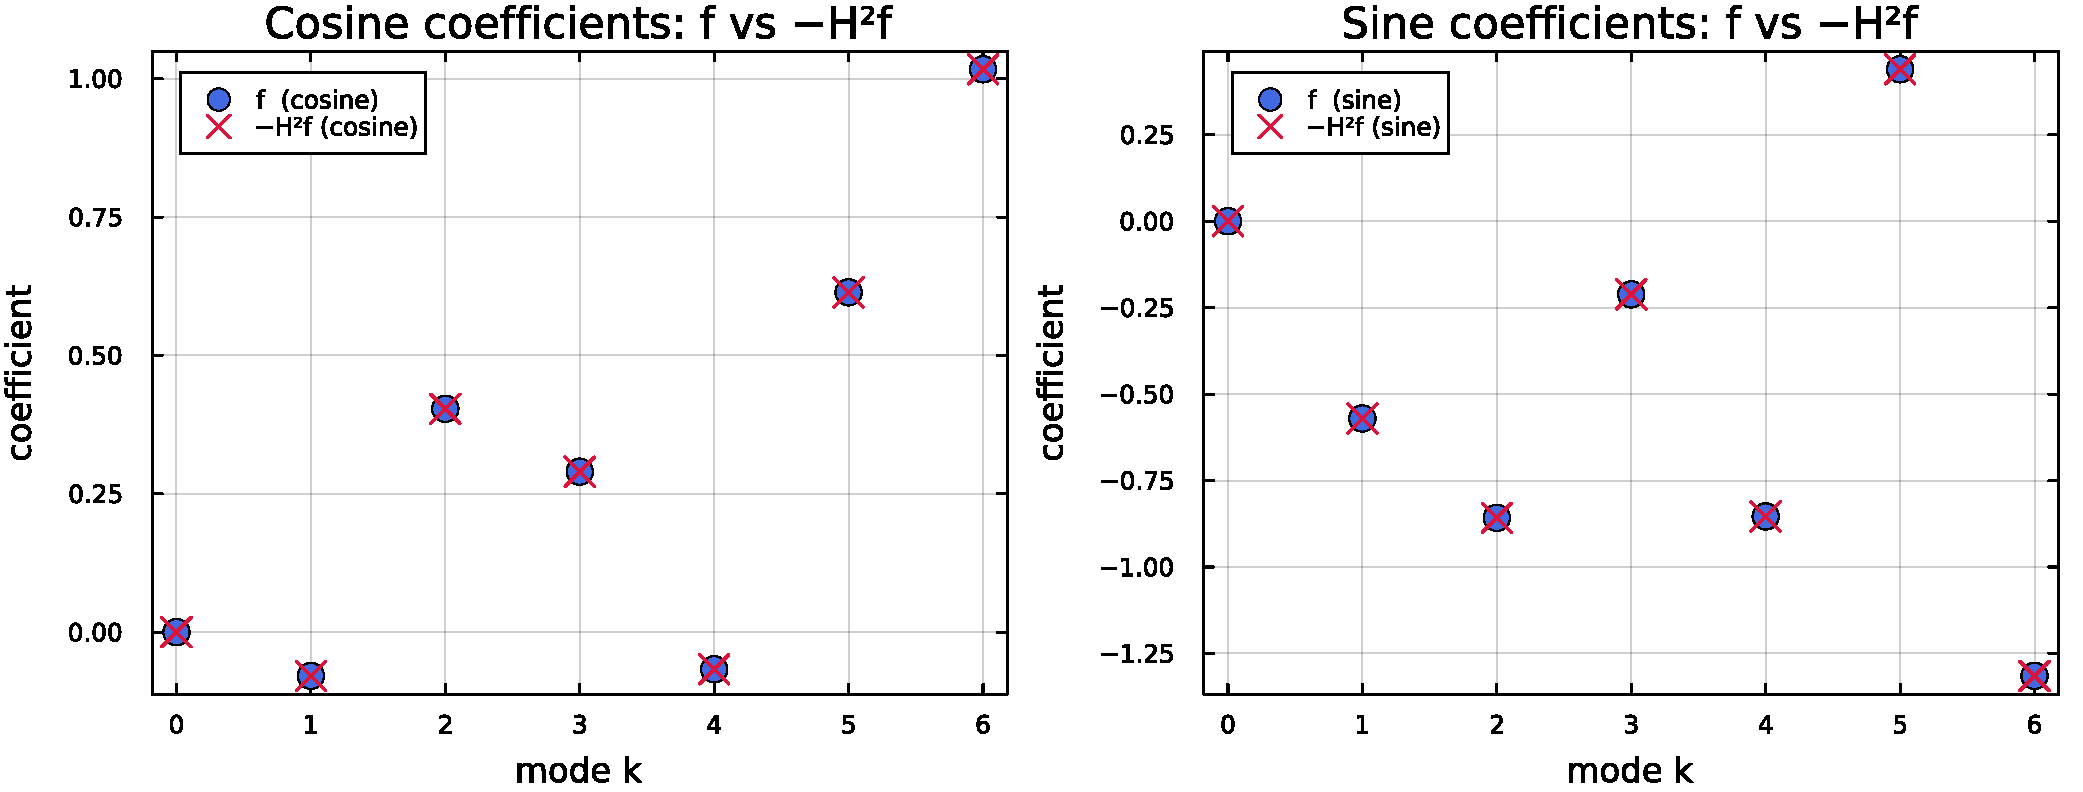
\includegraphics[width=\linewidth]{figures/fig2_hsquared.pdf}
  \caption{T1.1: Cosine (left) and sine (right) coefficients of a random
           degree-6 mean-zero trig poly $f$ (blue circles) and $-\hat H^2[f]$
           (red crosses). The markers coincide exactly at every mode,
           confirming $\hat H^2[f] = -f$ at the level of exact algebraic
           arithmetic.}
  \label{fig:hsquared}
\end{figure}

\subsection{Test T1.2: $\hat H$ and $\partial_u$ commute}

We verify \eqref{eq:commute}: $\hat H[\partial_u f] = \partial_u \hat H[f]$
for a random degree-6 polynomial.

\begin{lstlisting}
lhs = hilbert(deriv(f))    # H[f']
rhs = deriv(hilbert(f))    # (Hf)'
@test trigpoly_equal(lhs, rhs)
\end{lstlisting}

\textbf{Result: 5/5 assertions pass.}
Figure~\ref{fig:commutation} shows both sides overlaid (left panel, visually
indistinguishable) and the pointwise difference (right panel), which is at the
level of $10^{-38}$.

\begin{figure}[H]
  \centering
  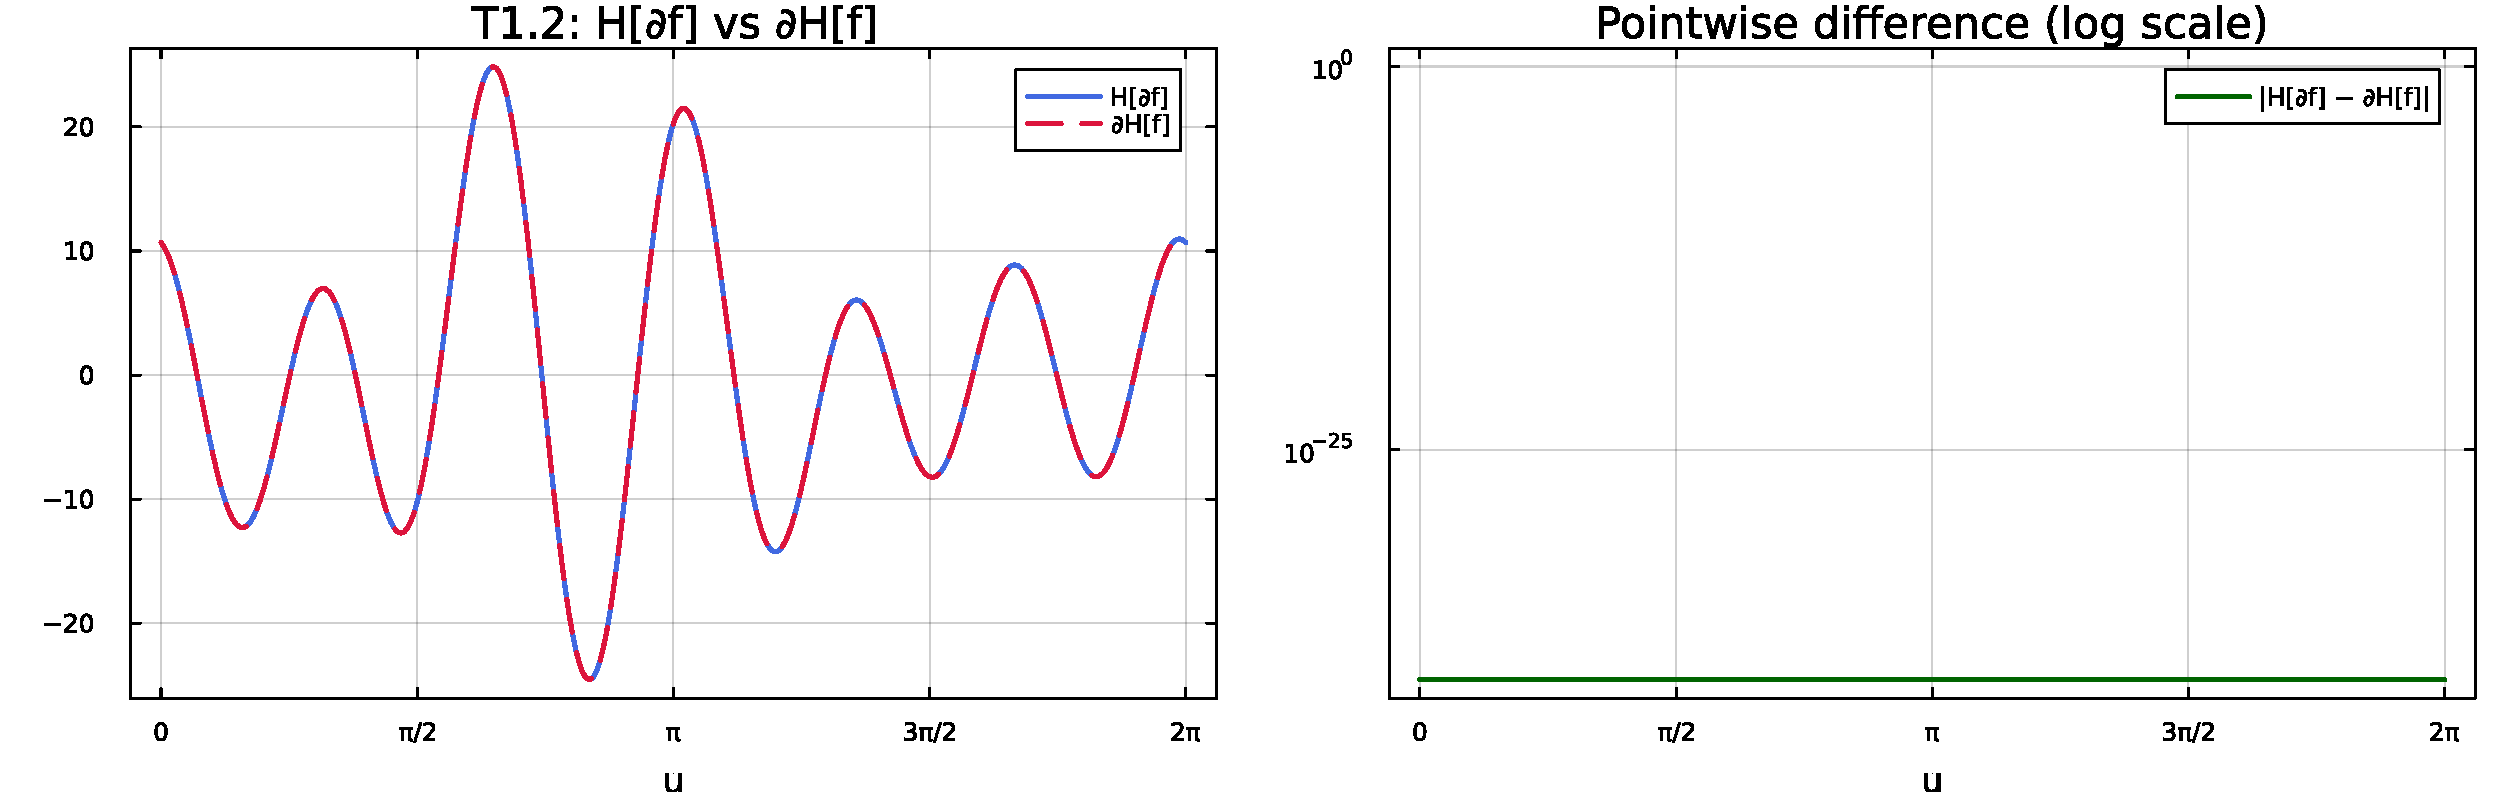
\includegraphics[width=\linewidth]{figures/fig3_commutation.pdf}
  \caption{T1.2: Left: $\hat H[\partial_u f]$ and $\partial_u \hat H[f]$
           overlaid — the curves are identical. Right: pointwise absolute
           difference (log scale), at the level of $10^{-38}$.}
  \label{fig:commutation}
\end{figure}

\subsection{Test T1.3: Supremum-norm bound is genuine}

We evaluate a random degree-8 polynomial at 1000 equally-spaced Arb points
and verify that every $|f(u_j)|$ is bounded by \texttt{supnorm\_bound}$(f)$.

\begin{lstlisting}
bound = supnorm_bound(f)
us = [Arb(2*pi*j/1000; prec) for j in 0:999]
@test all(Arblib.le(abs(tp_eval(f, u)), bound) for u in us)
\end{lstlisting}

\textbf{Result: 3/3 assertions pass.}
Figure~\ref{fig:supnorm} shows $f(u)$ against the bound (dashed red line).
The bound lies above the curve at all 1000 sample points.

\begin{figure}[H]
  \centering
  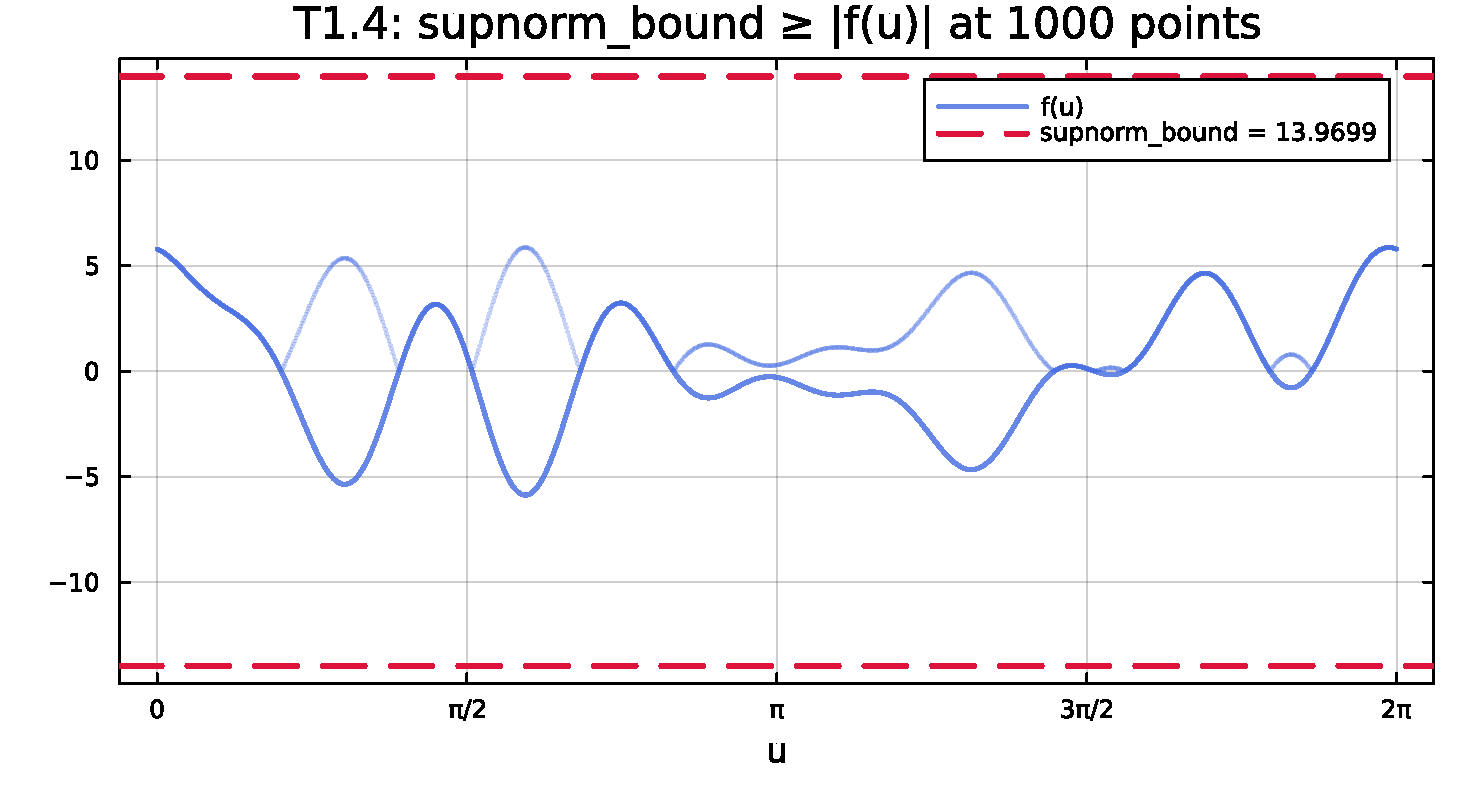
\includegraphics[width=0.75\linewidth]{figures/fig4_supnorm.pdf}
  \caption{T1.3: $f(u)$ at 1000 grid points (blue) and the certified
           \texttt{supnorm\_bound} (red dashed lines). The bound encloses
           the function at all sampled points.}
  \label{fig:supnorm}
\end{figure}

\subsection{Test T1.4: Agreement with Float64 baseline and coefficient-level rigor}

For $y(u) = 0.3\cos u + 0.15\cos 2u + 0.07\cos 3u$, we compare $\hat H[y_u]$
computed by \texttt{TrigPoly} (Arb) against the analytic Float64 formula
$\hat H[y_u](u) = \sum_k k\,a_k\cos(ku)$.
Since $y$ is a pure cosine series, $\hat H[y_u]$ is a pure cosine series
with known closed form, so no FFT or interpolation is involved in the reference.

The test has three parts:
(i) at 100 grid points, the Arb midpoint of $\hat H[\partial_u y]$ agrees with the
Float64 FFT reference to better than $10^{-13}$;
(ii) the Arb coefficient ball $\hat H[\partial_u y].a[k+1]$ \emph{overlaps} an
independent Arb computation of $k \cdot \texttt{Arb}(a_k)$ (integer multiplication
in Arb is exact, so this is a genuine rigor check on the \texttt{hilbert} and
\texttt{deriv} implementations, not a self-referential tautology);
(iii) the Arb midpoint matches the expected Float64 value $k \cdot a_k$ within
$10^{-15}$.

\textbf{Result: 7/7 assertions pass.}
Figure~\ref{fig:float64} shows both curves overlaid (left panel) and the
absolute error (right panel). All errors are below $10^{-13}$; the actual
errors are near $10^{-16}$, consistent with Float64 rounding of
$\cos(ku)$ at 100 evaluation points.

\begin{figure}[H]
  \centering
  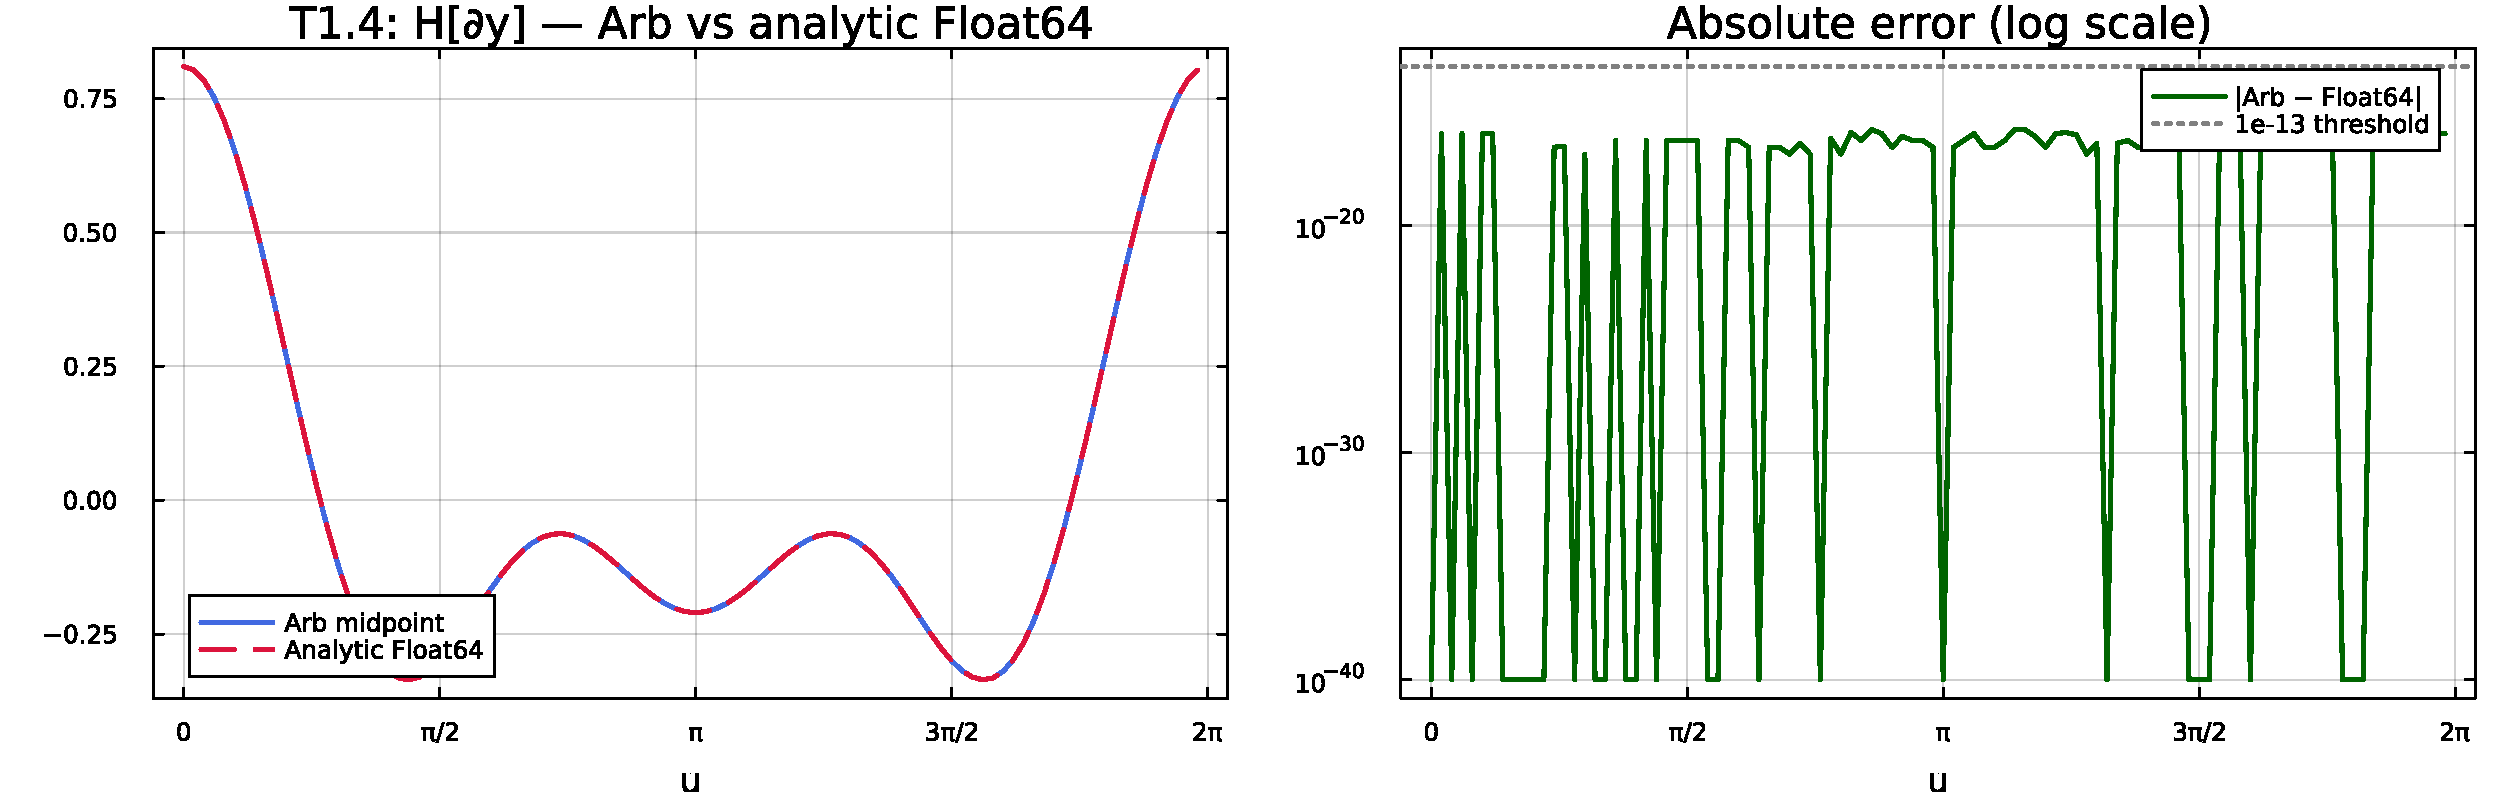
\includegraphics[width=\linewidth]{figures/fig5_float64_comparison.pdf}
  \caption{T1.4: Left: $\hat H[\partial_u y]$ computed by Arb
           \texttt{TrigPoly} (blue) and the analytic Float64 formula (red
           dashed) — indistinguishable at this scale. Right: pointwise
           absolute error (log scale). Errors are at the level of Float64
           rounding ($\sim 10^{-16}$), well below the $10^{-13}$ threshold.}
  \label{fig:float64}
\end{figure}

A representative plot of the Hilbert transform in action is shown in
Figure~\ref{fig:example}: a random degree-5 polynomial $f$ and its
Hilbert transform $\hat H[f]$, illustrating the $\pi/2$ phase shift
on each mode.

\begin{figure}[H]
  \centering
  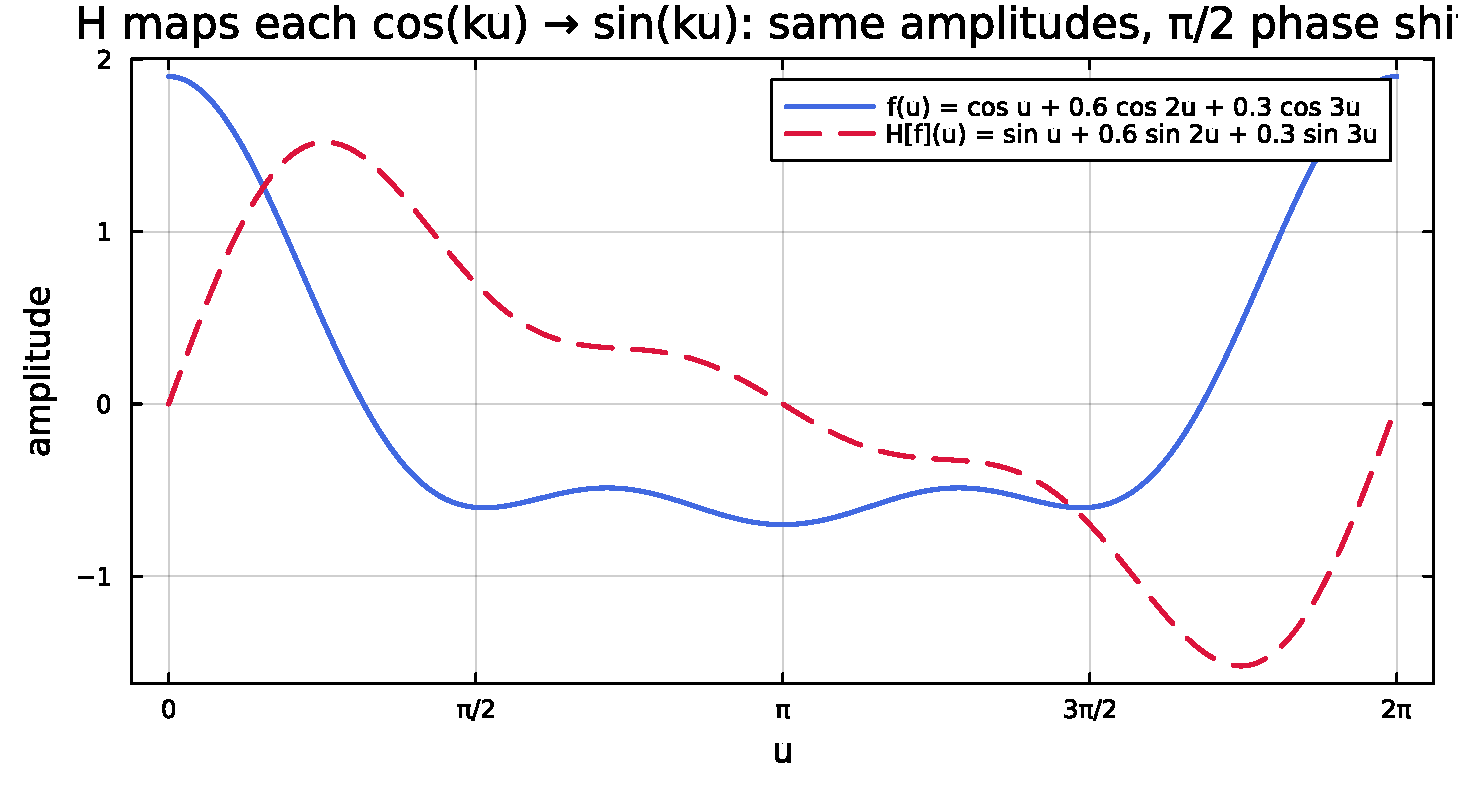
\includegraphics[width=0.75\linewidth]{figures/fig1_hilbert_example.pdf}
  \caption{$f(u) = \cos u + 0.6\cos 2u + 0.3\cos 3u$ (blue) and its
           Hilbert transform $\hat H[f](u) = \sin u + 0.6\sin 2u + 0.3\sin 3u$
           (red dashed). The two curves have identical mode amplitudes; $\hat H$
           shifts each cosine mode to the corresponding sine, i.e.\ a $\pi/2$
           phase shift per mode.}
  \label{fig:example}
\end{figure}

%% ─────────────────────────────────────────────────────────────────────────────
\section{Summary}

\begin{table}[H]
\centering
\begin{tabular}{llcc}
\toprule
Test & Description & Assertions & Result \\
\midrule
T1.1 & $\hat H^2 = -I$ on degree-8 random poly & 6 & \textcolor{green!60!black}{\textbf{pass}} \\
T1.2 & $\hat H \circ \partial_u = \partial_u \circ \hat H$ & 5 & \textcolor{green!60!black}{\textbf{pass}} \\
T1.3 & \texttt{supnorm\_bound} $\ge |f(u_j)|$ at 1000 points & 3 & \textcolor{green!60!black}{\textbf{pass}} \\
T1.4 & Arb midpoint agrees with analytic Float64 to $< 10^{-13}$; coefficient
       overlap against independent Arb computation & 7 & \textcolor{green!60!black}{\textbf{pass}} \\
Sanity & $b_0 = 0$ after every op & 5 & \textcolor{green!60!black}{\textbf{pass}} \\
Sanity & \texttt{cosine\_series} constructor & 5 & \textcolor{green!60!black}{\textbf{pass}} \\
\midrule
\textbf{Total} & & \textbf{31} & \textcolor{green!60!black}{\textbf{31/31}} \\
\bottomrule
\end{tabular}
\caption{M1 test summary. All 31 assertions pass at 128-bit Arb precision.}
\end{table}

Milestone M1 is complete. The \texttt{FourierSeries.jl} module provides a
correct, certified foundation for the downstream Julia milestones:
\begin{itemize}
  \item \textbf{M2} (\texttt{TaylorSeries.jl}) evaluates \texttt{TrigPoly}
        objects at Arb grid points and builds certified Taylor series for
        non-polynomial quantities such as $D$, $1/D$, and $G = (1+\hat H[y_u])/D$.
        It also provides \texttt{dmin\_bound}, the certified lower bound on $D$.
  \item \textbf{M3} (\texttt{GDerivatives.jl}) computes $G^{(m)}(u_j)$ at each
        grid point using M2's Taylor series machinery.
  \item \textbf{M5/M6} (\texttt{ResidualBound.jl}) assembles all terms of the
        Babenko residual. Products such as $y \cdot \hat H[y_u]$ are computed
        pointwise at grid points; the symbolic \texttt{TrigPoly} layer handles
        only $\hat H$ and $\partial_u$.
\end{itemize}

\end{document}
